
\paragraph{}
\large in this section, we start making a review of the most common techniques usually used in Facial Expression Detection, highlight methodological differences, discuss the reported performances and the dataset used. \newline

\textbf{Based on CNN and Fer 2013 Dataset}\newline

\large CNN has enabled significant performance improvements in related tasks specifically those dealing with images using CNN help in feature extraction and inference. 

\large FER2013 is a large, publicly available Facial Expression Detection dataset consisting of 35,887 face crops. The dataset is challenging as the depicted faces vary significantly in terms of person age, face pose, and other factors, reflecting realistic conditions. The dataset is split into training, validation, and test sets with 28,709, 3,589, and 3,589 samples, respectively. Basic expression labels are provided for all samples. All images are grayscale and have a resolution of 48 by 48 pixels. The human accuracy on this dataset is around 65.5\%.
  
\large Facial Expression Recognition using Convolutional Neural Networks: State of the Art paper\cite{state_of_art} get with only CNN 75\% testing accuracy.
also in this paper\cite{state_of_art} a detailed review of six models we only mention there Architecture and accuracy here. in table 2.2.1.
\begin{table}[h!]
	\begin{center}
		\caption{CNN ARCHITECTURES. C, P, N, I, AND F STANDS FOR CONVOLUTION,POOLING,NORMALIZATION,INCEPTION AND FULLY CONNECTED LAYERS, RESPECTIVELY. \newline}
		\label{tab:table 2.2.1}
		\begin{tabular}{l|c}
			\textbf{Method} & \textbf{Architecture} \\
			\hline
			method 1\cite{method_1} & CPCPFF \\
			method 2\cite{method_2} & CPCPCPFF \\
			method 3\cite{method_3} & PCCPCCPCFFF \\
			method 4\cite{method_4} & CPCPIIPIPFFF \\
			method 5\cite{method_5} & CPNCPNCPCFF \\						
			method 6\cite{method_6} & CPCPCPFF \\
		\end{tabular}

	\end{center}
		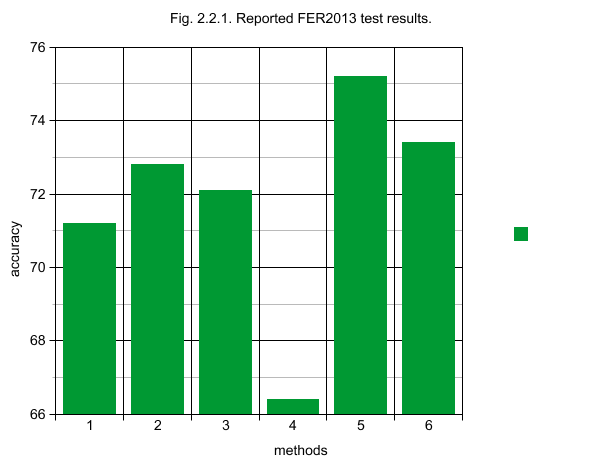
\includegraphics[scale=0.3]{graph.png}
\end{table}
 % <-- i will edit graphs i do not know how to put side by side 
\paragraph{}
\large the biggest bottleneck here according to paper is the dataset as it has an only 35k image with a lot of noise and needs too much preprocessing the quick solution for it is appling data augmentation with different attributes.

\large another model build over state of art try to overcome its discussed problem is applied the model on tensorflow and CNN also work on fer13 . it defines a similar method to the final methods with some addition to help improve dataset performance adding Dropout and normalization Layers and it uses landmarks and a sliding window Hog as feature extraction. \newline
Also we found an implementation using SVM, it depends actually on extraction features using landmarks and Hog and feeds them to a multi-class SVM classifier.here we can find the different architecture and accuracy of two models based on CNN and SVM model.

\begin{table}[h!]
	\begin{center}
		\caption{3. Classification Results (training on 5 expressions)\newline}
		\label{tab:table 2.2.2}
		\begin{tabular}{l|c|l|l}
			\textbf{Experiments} & \textbf{SVM}   & \textbf{Model A}   & \textbf{Model B}  \\
			\hline
			CNN (on raw pixels)	& -----   & 72.4\% & 73.5\% \\ 
			CNN + Face landmarks & 46.9\% &	73.5\% & 74.4\% \\
			CNN + Face landmarks + HOG & 55.0\% & 68.7\% & 73.2\% \\
			CNN + Face landmarks + HOG + sliding window & \textbf{59.4\%} &\textbf{71.4\%}&\textbf{75.1\%}\\
		& & 
		\end{tabular}
		
	\end{center}
	\includegraphics[scale=0.3]{cnn_arch_amine.png}
\end{table}
% <-- i will edit graphs 
\large we try this model with this architecture (model B), the same preprocessing and on the same dataset but we get only 50\% testing accuracy.





